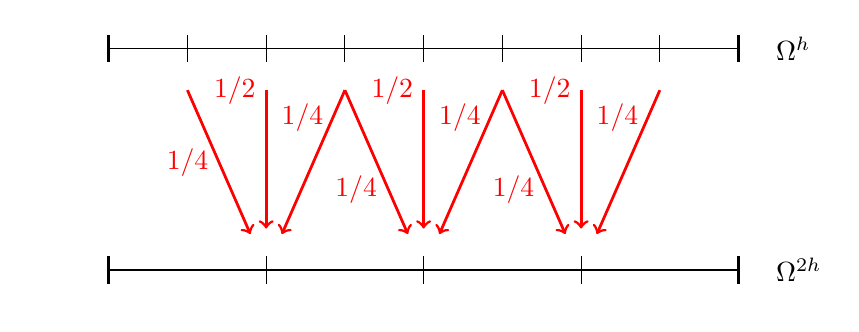
\begin{tikzpicture}
    \draw (0, 0) node[left]{\phantom{$\quad \Omega^{h}$}} -- (8, 0) node[right]{$\quad \Omega^{h}$};
    \draw[line width = 1pt] (0, .5em) -- (0, -.5em) node[below] {} ;
    \draw[line width = 1pt] (8, .5em) -- (8, -.5em) node[below] {} ;
    \foreach \x in {1, ..., 7}
        \draw[shift={(\x, 0)}] (0, .5em) -- (0, -.5em);

    \draw (0, -8em) node[right]{\phantom{$\quad \Omega^{2h}$}}-- (8, -8em) node[right]{$\quad \Omega^{2h}$};
    \draw[line width = 1pt] (0, -7.5em) -- (0, -8.5em) node[below] {} ;
    \draw[line width = 1pt] (8, -7.5em) -- (8, -8.5em) node[below] {} ;
    \foreach \x in {2, 4, 6}
        \draw[shift={(\x, 0)}] (0, -7.5em) -- (0, -8.5em);
    
    {
    \color{red}
    %% n = 1
    \draw[->, line width=1pt] 
    (1, -1.5em) 
    -- 
    (1.8, -6.7em) node[midway, left]{1/4} ;
    \draw[->, line width=1pt] 
    (2, -1.5em) node[left]{1/2} 
    -- 
    (2, -6.5em)
    ;
    \draw[->, line width=1pt] 
    (3, -1.5em) node[left, yshift=-1em, xshift=-.4em]{1/4} 
    -- 
    (2.2, -6.7em)  ;
    
    %% n = 4
    \draw[->, line width=1pt] 
    (3, -1.5em) 
    -- 
    (3.8, -6.7em) node[midway, left, yshift=-1em, xshift=.4em]{1/4} ;
    \draw[->, line width=1pt] 
    (4, -1.5em) node[left]{1/2} 
    -- 
    (4, -6.5em)
    ;
    \draw[->, line width=1pt] 
    (5, -1.5em) node[left, yshift=-1em, xshift=-.4em]{1/4} 
    -- 
    (4.2, -6.7em)  ;
    
    %% n = 6
    \draw[->, line width=1pt] 
    (5, -1.5em) 
    -- 
    (5.8, -6.7em) node[midway, left, yshift=-1em, xshift=.4em]{1/4} ;
    \draw[->, line width=1pt] 
    (6, -1.5em) node[left]{1/2} 
    -- 
    (6, -6.5em)
    ;
    \draw[->, line width=1pt] 
    (7, -1.5em) node[left, yshift=-1em, xshift=-.4em]{1/4} 
    -- 
    (6.2, -6.7em)  ;
    }
\end{tikzpicture}
